\begin{figure}[!ht]
\centering
\noindent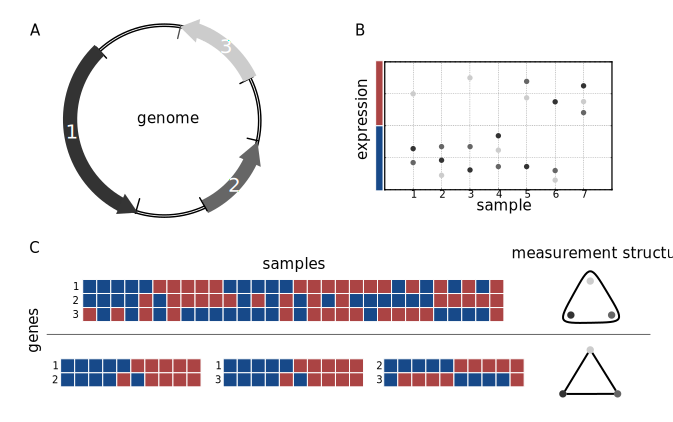
\includegraphics[width=0.9\columnwidth]{fig/figure_expression_concept.pdf}
\caption{{\bf Coarse-graining of gene expression data.}}
\label{fig:expression_concept}
\end{figure}

\begin{figure}[!ht]
\centering
\noindent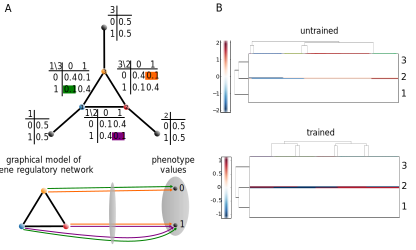
\includegraphics[width=0.9\columnwidth]{fig/inconsistentthreecycle.pdf}
\caption{{\bf Probabilistic graphical model of inconsistent gene expression data.}}
\label{fig:inconsistentthreecycle}
\end{figure}

\begin{figure}[!ht]
\centering
\noindent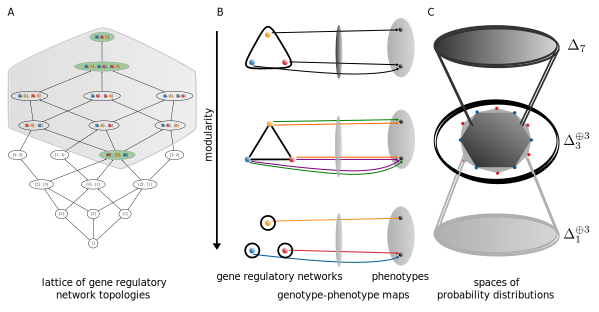
\includegraphics[width=0.9\columnwidth]{fig/conediagram.pdf}
\caption{{\bf Relationship between gene regulatory network models and spaces of probability distributions.}}
\label{fig:conediagram}
\end{figure}

\begin{figure}[!ht]
\centering
\noindent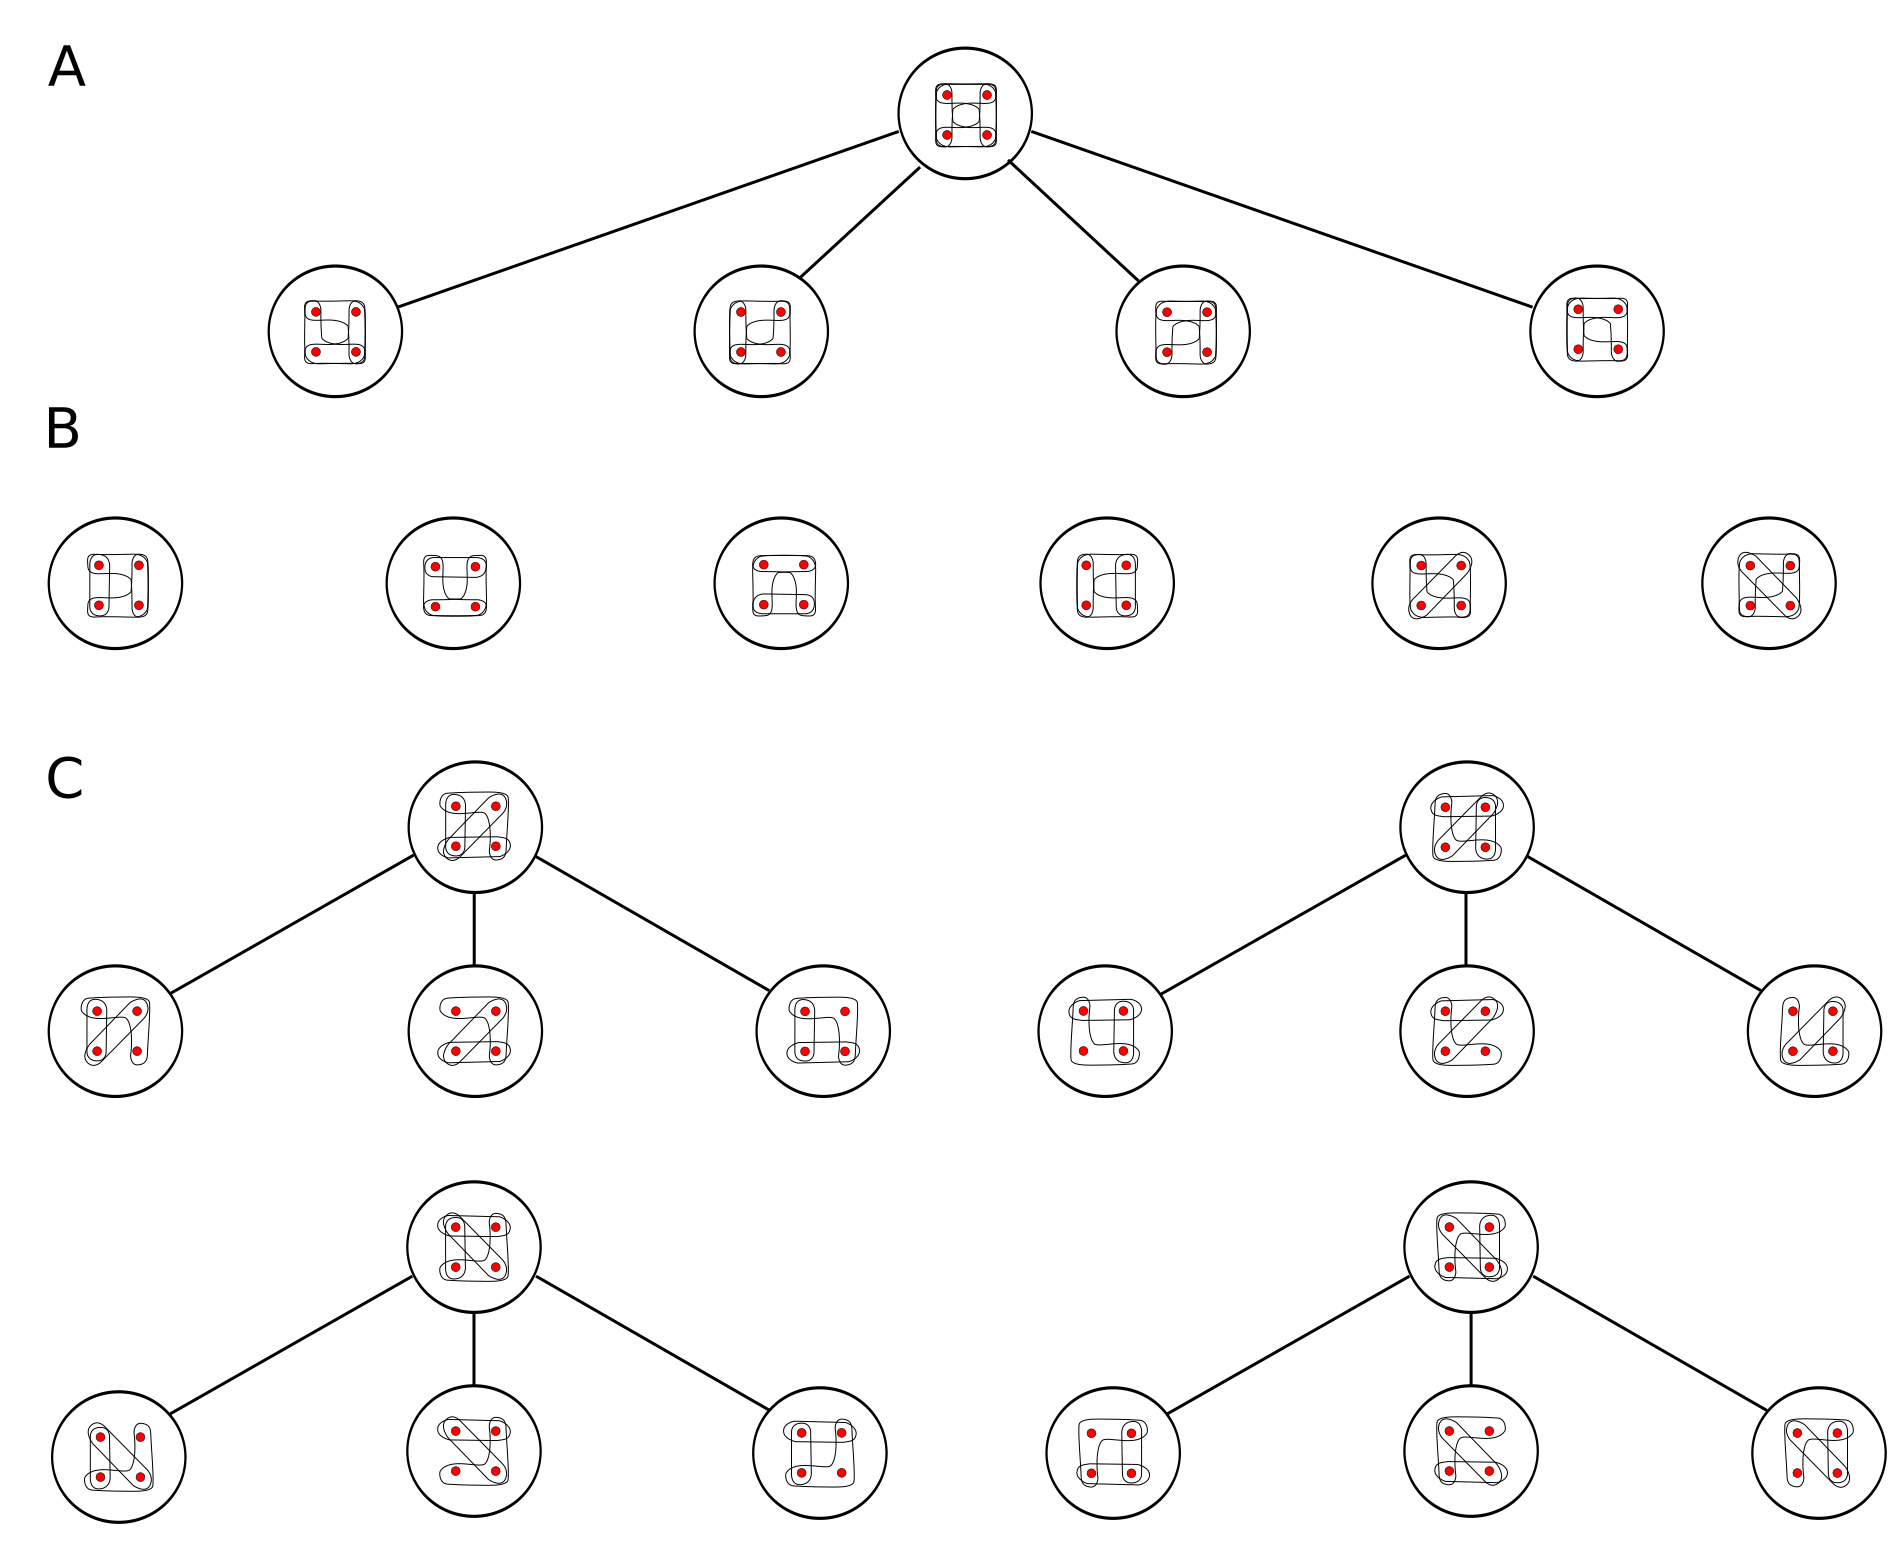
\includegraphics[width=0.9\columnwidth]{fig/non2uniformcyclichypergraphhasse.pdf}
\caption{{\bf Hierarchical relationships among all possible classes of hypergraphs that are not graphs (i.e. not 2-uniform) but have cycles.}}
\label{fig:non2uniformcyclichypergraphhasse}
\end{figure}

\begin{figure}[!ht]
\centering
\noindent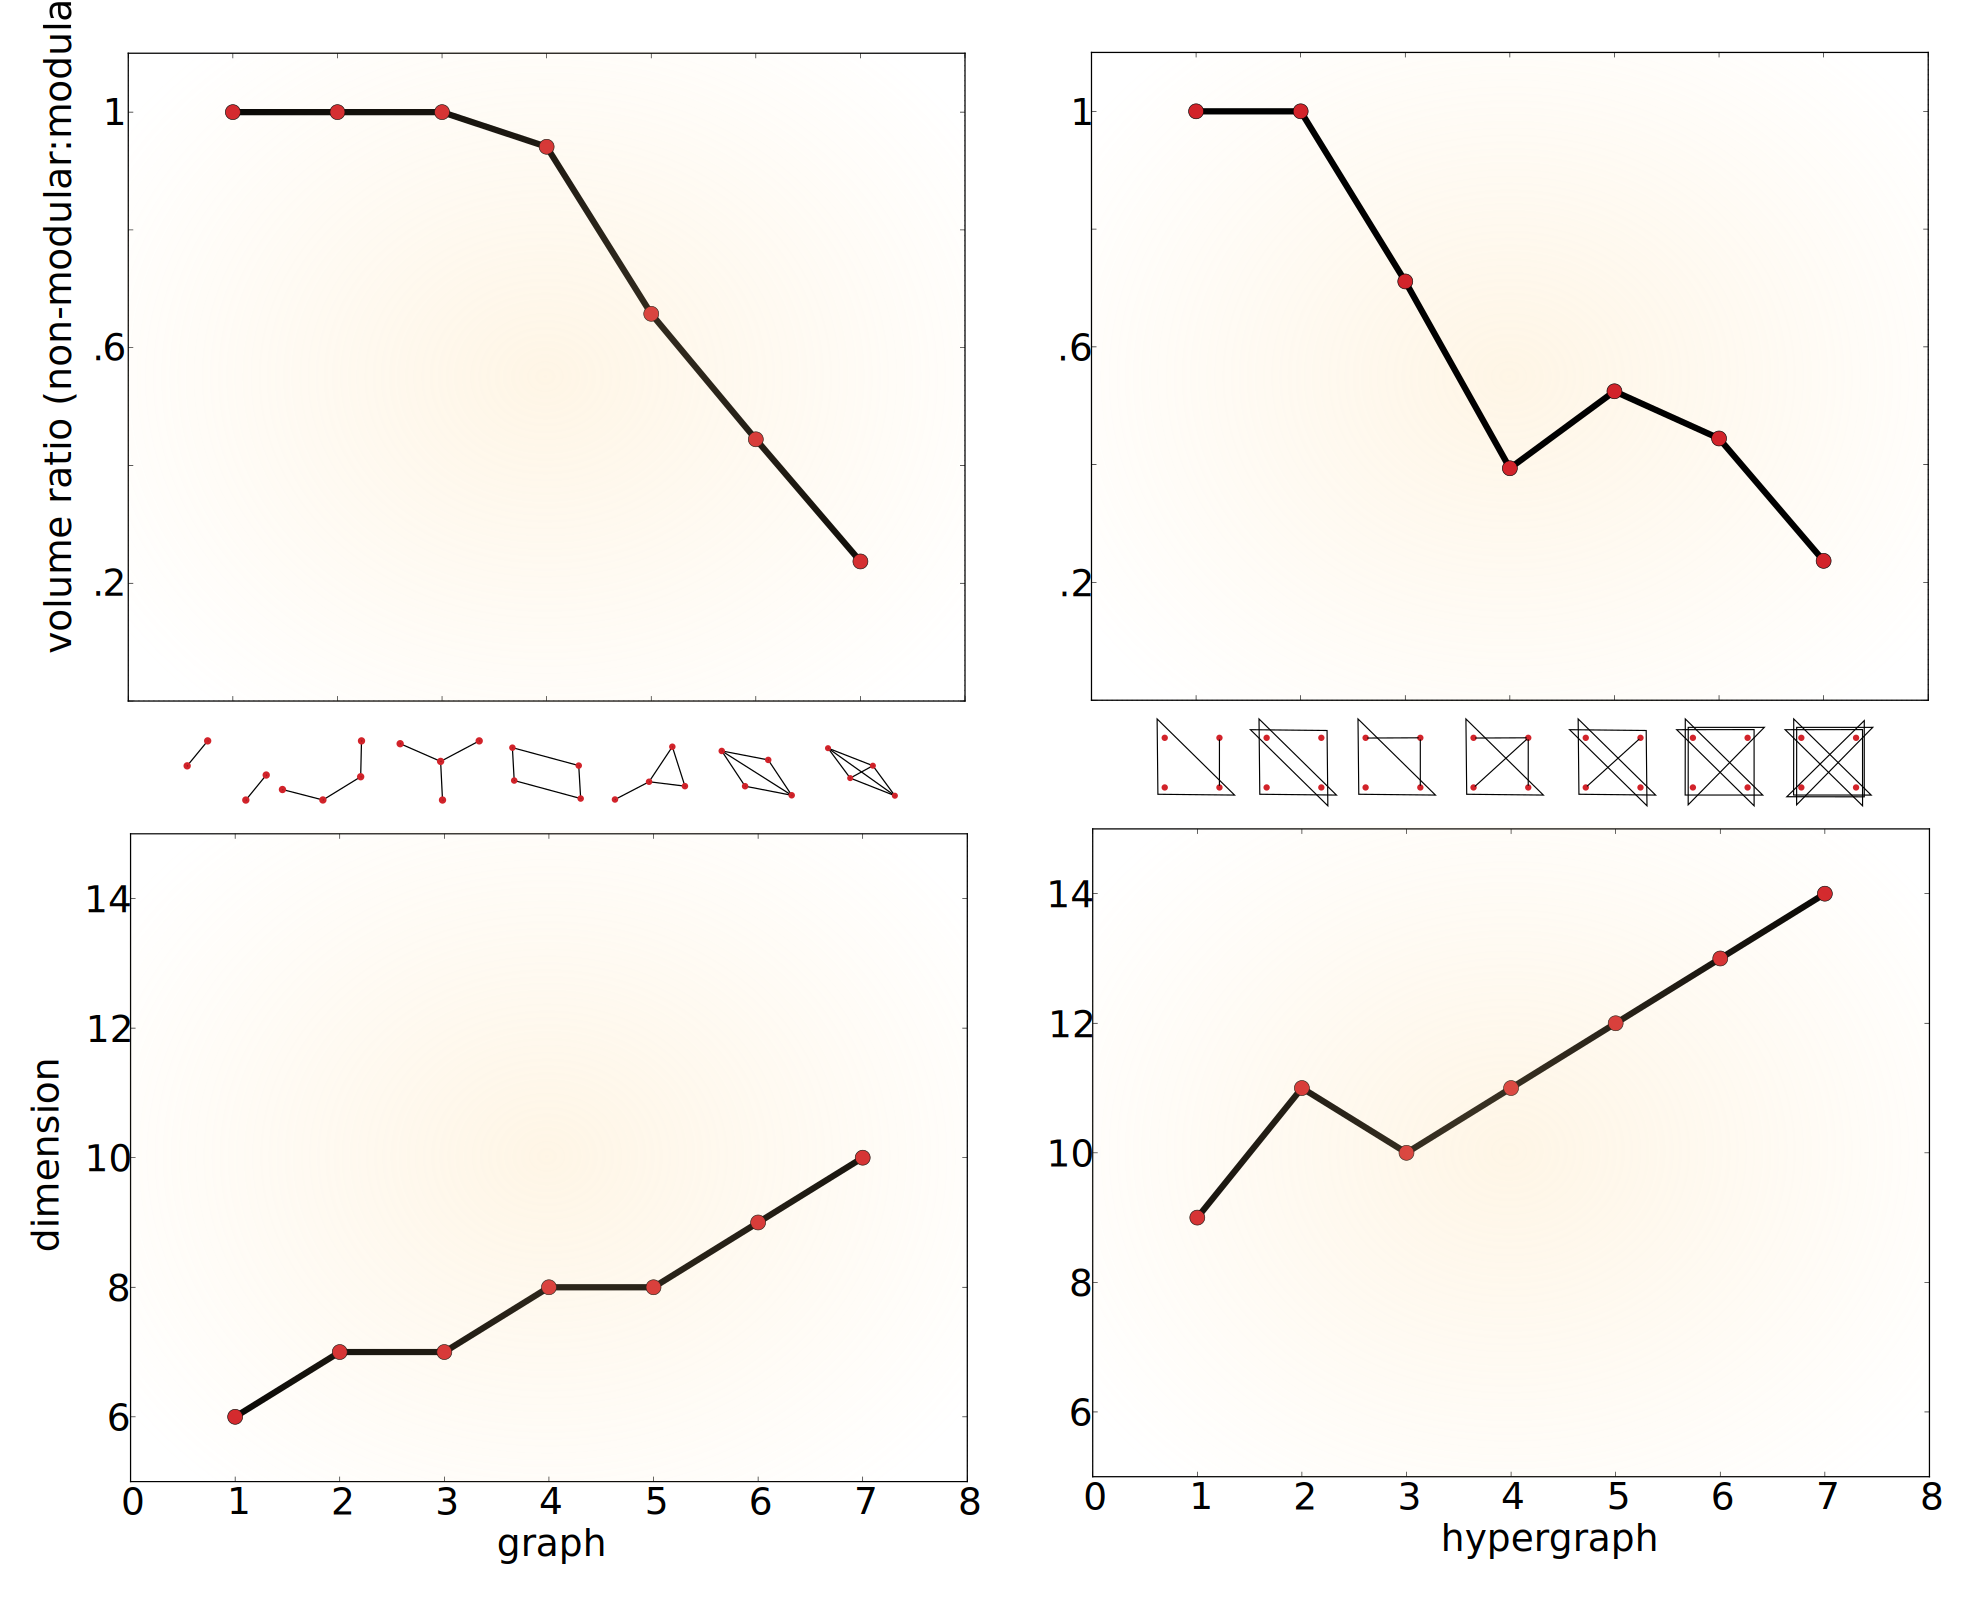
\includegraphics[width=0.9\columnwidth]{fig/figure_graphs_dims_nolines.pdf}
\caption{{\bf Non-modular to modular probability space volume ratio.}}
\label{fig:ncycvolrat}
\end{figure}

\begin{figure}[!ht]
\centering
\noindent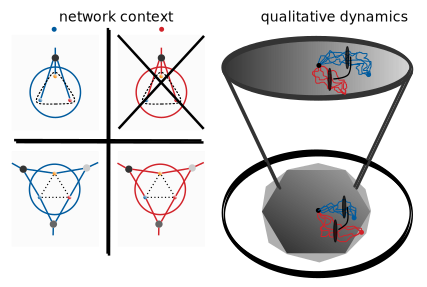
\includegraphics[width=0.9\columnwidth]{fig/stochdynscheme.pdf}
\caption{{\bf Schematic representation of the constraints imposed on stochastic gene expression and evolutionary dynamics by network architecture .}}
\label{fig:stochdynscheme}
\end{figure}
